
\definecolor{tnred}{RGB}{     255, 63,   63}
%\definecolor{tnorange}{RGB}{  255, 204,   6}
% #ecb939	()
\definecolor{tnorange}{RGB}{  220, 140,   6}
\definecolor{tnblue}{RGB}{     10, 154, 215}
\definecolor{tngreen}{RGB}{   114, 165,  10}
\definecolor{tnmagenta}{RGB}{ 215,  10, 154}
\definecolor{tnbg}{RGB}{252,252,252}
\definecolor{tnfg}{RGB}{5,8,12}



\tikzset{highlight/.style={orange!75!white,line width=6pt,line cap=round}}
\tikzset{highlight2/.style={tngreen!70!yellow!60,line width=11pt,line cap=round}}
\tikzset{psline/.style={decorate,decoration={amplitude=0.3mm,segment length=2mm,post length=1.5mm,pre length=1.5mm,coil,aspect=0}}}
\tikzset{plainlin/.style={line width=1pt}}
\def\shortendistance{5pt}
\tikzset{plainlin shorten/.style={line width=1pt,shorten >=\shortendistance,shorten <=\shortendistance}}

\tikzset{lin shorten/.style={shorten >=\shortendistance,shorten <=\shortendistance,line width=1pt,decoration={markings, mark=at position 0.5*\pgfdecoratedpathlength+1.8pt with {\arrow{angle 90}}}, postaction={decorate}}}
% Name of file with picture %%%%%%%%%%%%%%%%%%%%%%%%%%%%%%%%%%%%%%%%%%%
\tikzsetnextfilename{fig-separation}% <==================================


\newcommand{\vertexat}[1]{\fill [very thick,draw=white,fill=black] #1 circle (3pt);}


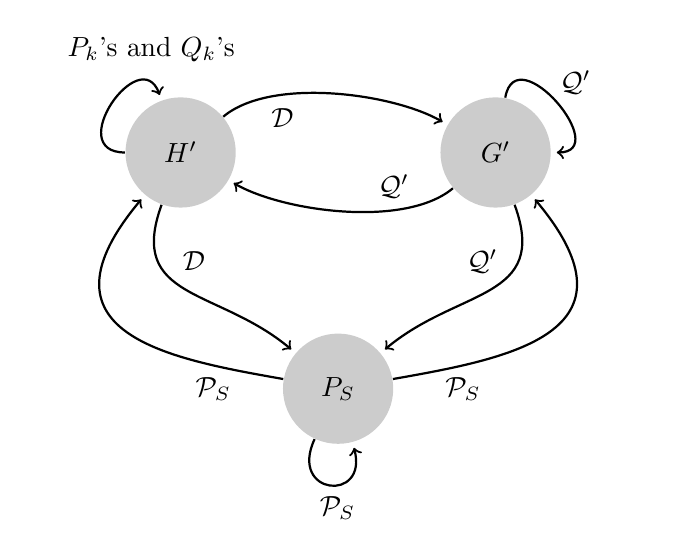
\begin{tikzpicture}
  \node[shape=circle,fill=gray!40,minimum size=1.4cm] (H')  at (-2, 0)    {$H'$};
  \node[shape=circle,fill=gray!40,minimum size=1.4cm] (G')  at ( 2, 0)    {$G'$};
  \node[shape=circle,fill=gray!40,minimum size=1.4cm] (PS) at ( 0,-3) {$P_S$};

   \begin{scope}[->, shorten >=2pt,thick]
     \draw (H') .. controls +(180:1.5cm) and +(110:1.5cm) .. node [midway,xshift=.5cm,yshift=.7cm] {$P_k$'s and $Q_k$'s} (H');
    % \draw (H') .. controls +(180:1.5cm) and +(110:1.5cm) .. node [midway,xshift=.5cm,yshift=.7cm] {$P_k \cup Q_k$} (H');
    % \draw (H') .. controls +(180:1.5cm) and +(110:1.5cm) .. node [midway,xshift=.5cm,yshift=.7cm] {$P_1,\dots,P_{2n},Q_1,\dots,Q_{3n}$} (H');
    % \draw (H') .. controls +(180:1.5cm) and +(110:1.5cm) .. node [midway,xshift=-1.3cm,yshift=.2cm] {\parbox{2cm}{\,\,\,\,$P_1,\dots,P_{2n}$\newline$Q_1,\dots,Q_{3n}$}} (H');

    \draw (G') .. controls +(80:1.5cm) and +(0:1.5cm) .. node [midway,xshift=.25cm,yshift=.25cm] {$\mathcal{Q}'$} (G');


    % Loop below PS
    \draw (PS) .. controls +(-115:1.5cm) and +(-75:1.5cm) .. node [midway,xshift=0.1cm,yshift=-.3cm] {$\mathcal{P}_S$} (PS);
    % Loop above PS
    % \draw (PS) .. controls +(115:1.5cm) and +(75:1.5cm) .. node [midway,xshift=0.05cm,yshift=.25cm] {$\mathcal{P}_S$} (PS);

    \draw (H') .. controls +(40:1.5cm) and +(150:1.5cm) ..  node [pos=.3,yshift=-.3cm] {$\mathcal{D}$}  (G');
    \draw (G') .. controls +(220:1.5cm) and +(-30:1.5cm) ..  node [pos=.3,yshift=.3cm] {$\mathcal{Q}'$}  (H');


    \draw (H') .. controls +(-110:2cm) and +(140:2cm) ..  node [pos=.45,yshift=.3cm,xshift=.2cm] {$\mathcal{D}$}  (PS);
    \draw (PS) .. controls +(170:2.2cm) and +(-130:3cm) ..  node [pos=.2,yshift=-.3cm] {$\mathcal{P}_S$}  (H');


     \draw (G') .. controls +(-70:2cm) and +(40:2cm) ..  node [pos=.45,yshift=.3cm,xshift=-.2cm] {$\mathcal{Q}'$}  (PS);
     \draw (PS) .. controls +(10:2.2cm) and +(-50:3cm) ..  node [pos=.2,yshift=-.3cm] {$\mathcal{P}_S$}  (G');

    % \coordinate (aux1) at ($(H') + (-105:2.2cm)$);
    % \coordinate (aux2) at ($(PS) + (110:2cm)$);

    % \useasboundingbox (H') (PS) (G');
 \end{scope}

\end{tikzpicture}